\documentclass[11pt]{article}

\usepackage[margin=1in]{geometry}
\usepackage{amsmath, amssymb}
\usepackage{booktabs}
\usepackage{graphicx}
\usepackage{siunitx}
\usepackage{hyperref}
\usepackage{xcolor}
\usepackage{listings}

\emergencystretch=2em

\lstset{
  language=Python,
  basicstyle=\small\ttfamily,
  keywordstyle=\bfseries,
  commentstyle=\itshape\color{gray},
  showstringspaces=false,
  breaklines=true,
  columns=fullflexible,
  frame=single,
  framesep=4pt,
  xleftmargin=4pt,
  xrightmargin=4pt,
}

\newcommand{\lamd}{\lambda_{\mathrm{deriv}}}
\newcommand{\lamb}{\lambda_{\mathrm{boundary}}}
\newcommand{\lama}{\lambda_{\mathrm{amp}}}
\newcommand{\lamdisc}{\lambda_{\mathrm{disc}}}

\title{Choosing the GRAPE Penalty Weights\\
\large A Pareto Sweep Under a Hardware Bandwidth Budget}
\author{}
\date{}

\begin{document}
\sloppy
\maketitle

\section{Motivation}
\label{sec:motivation}

The cost function that trains every logical-gate pulse in this project is not just a fidelity.
It is a fidelity plus four penalty terms:
%
\begin{equation}
\label{eq:cost}
\mathcal{C}(u) \;=\; -\,\overline{F_{\mathrm{coh}}}(u)
\;+\; \lamdisc \sum_{i \neq j} \bigl(F_i - F_j\bigr)^2
\;+\; \lamd\, g_{d}(u)
\;+\; \lamb\, g_{b}(u)
\;+\; \lama\, g_{a}(u),
\end{equation}
%
where $\overline{F_{\mathrm{coh}}}$ is the coherent process fidelity averaged over the training
truncations (Heeres et al.\ Supp.\ Eq.~23), the $\lamdisc$ term is the cross-truncation
discrepancy penalty (Supp.\ Eq.~24), and $g_d, g_b, g_a$ are the derivative, boundary, and soft
amplitude penalties defined in \texttt{core/grape\_core.py}.

Every penalty term in Eq.~\eqref{eq:cost} is non-negative and can only \emph{raise} the cost.
That has an uncomfortable consequence: if the four weights are tuned to maximize the training
objective, the tuning will drive all four to zero. The optimizer will happily oblige, and it will
return a pulse that is rougher, wider in bandwidth, and better at exploiting the finite
Hilbert-space truncation it was trained on. The training number goes up; the pulse gets worse.

So the weights cannot be chosen by optimizing the same quantity the weights appear in. They have
to be chosen against something training never sees. This report does that in three steps: it
sweeps the weights, scores each candidate on the \emph{reported} gate fidelity over
\emph{held-out} cavity truncations, and then picks a recipe subject to a hardware bandwidth
budget.

\section{What is measured}
\label{sec:metrics}

The distinction that matters throughout is between the \textbf{training objective} and the
\textbf{reported metric}.

\begin{itemize}
  \item $F_{\mathrm{coh}}$ --- the coherent process fidelity the optimizer actually descends on,
        evaluated at the training truncations $n_c \in \{22, 24, 26\}$. This is what
        \texttt{optimize\_multi\_state\_pulse} returns.
  \item $F_{\mathrm{held}}$ --- the Pedersen gate fidelity, computed from the \emph{full} $D
        \times D$ propagator, projected onto the logical subspace
        ($\texttt{logical\_block} = B^{\dagger} U B$), and evaluated at cavity truncations
        \emph{not} used in training. This is the headline number, produced by
        \texttt{main.report\_pedersen\_gate\_fidelity}.
\end{itemize}

Alongside the fidelity, each candidate carries pulse-cost and robustness metrics:
the RMS spectral bandwidth of the wider of the two drives, the peak drive amplitude, a
per-step roughness (RMS first difference), the spread $\max - \min$ of $F_{\mathrm{held}}$
across the held-out set, and the mean leakage $L_1$ out of the logical subspace.

\subsection{Experimental design}

Only the four $\lambda$'s vary. Everything else --- the smooth random warm start, the training
truncations $[22,24,26]$, the hard frequency bands ($\pm\SI{27}{\mega\hertz}$ cavity,
$\pm\SI{33}{\mega\hertz}$ transmon), the amplitude limits (\num{40} rad/$\mu$s), $N = 550$, and
$\mathrm{d}t = \SI{2}{\nano\second}$ --- is pinned in \texttt{analysis.penalty\_sweep.FIXED}.
Two search modes are used: a one-factor-at-a-time (OFAT) ladder over each axis in turn with the
others at their incumbent values, and a focused two-dimensional grid over $\lamd \times \lamb$.
The OFAT axes are $\lamd$, $\lamb$, $\lamdisc$, and the amplitude \emph{threshold}
$\epsilon_{\max}$; the reason $\epsilon_{\max}$ appears in place of the weight $\lama$ is given
in Section~\ref{sec:inert}.

Because L-BFGS-B on this landscape is non-convex, each configuration is trained from several
random seeds and the figures carry the across-seed standard deviation. A fidelity gap smaller
than that spread is not a ranking.

\section{Results}
\label{sec:results}

\subsection{One-factor-at-a-time response}

\IfFileExists{figures/penalty_ofat.pdf}{%
  \begin{figure}[htbp]
    \centering
    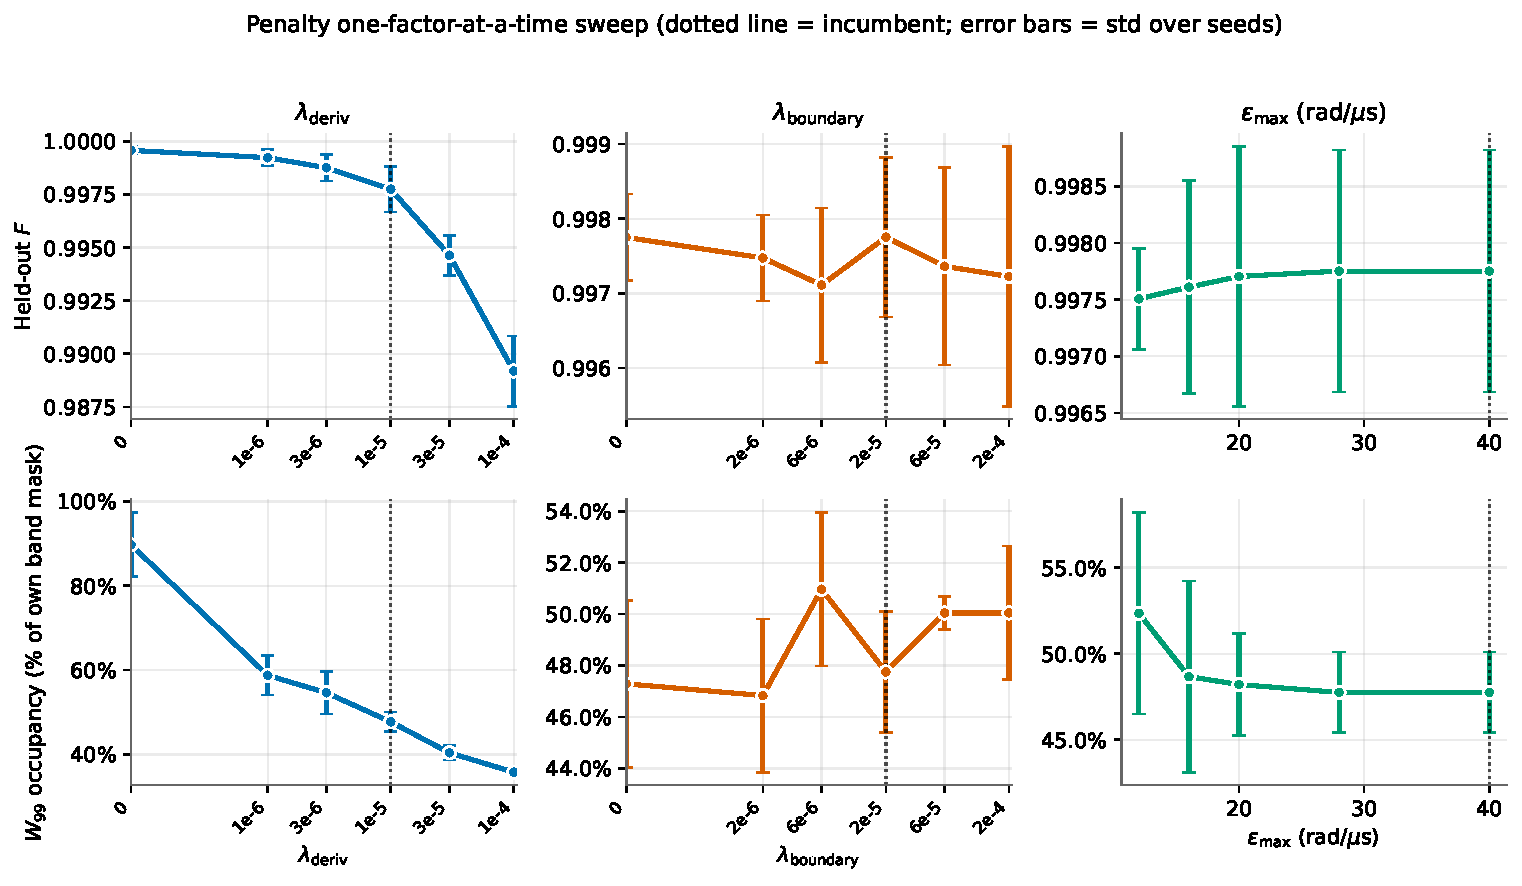
\includegraphics[width=\textwidth]{figures/penalty_ofat.pdf}
    \caption{Response of the reported held-out fidelity (top row) and the RMS pulse bandwidth
    (bottom row) as each penalty weight is varied with the other three held at the incumbent
    recipe. The dotted vertical line marks the incumbent value; error bars are the standard
    deviation across seeds. The leftmost point of each ladder is the $\lambda = 0$ negative
    control. Fidelity and bandwidth are plotted on separate rows rather than a shared twin axis,
    because the two scales are not commensurate.}
    \label{fig:ofat}
  \end{figure}
}{\emph{[Figure \texttt{figures/penalty\_ofat.pdf} not found --- run the sweep and
Section 3 of \texttt{penalty\_optimization.ipynb}.]}}

The $\lambda = 0$ rows are the control that makes the whole exercise meaningful. If removing a
penalty raised the training fidelity without costing anything measurable in bandwidth,
robustness, or peak amplitude, then that penalty was doing no work and belongs out of
Eq.~\eqref{eq:cost} entirely.

\subsection{Two of the four weights are inert}
\label{sec:inert}

The sweep's first substantive result is negative, and it is worth stating before anything else
because it changes what the remaining figures can possibly show. Two of the four weights in
Eq.~\eqref{eq:cost} have no effect under these conditions. Both were confirmed at convergence
against the canonical production pulse \texttt{pulses/u\_X\_main.npy}, not merely in an
under-trained regime.

\paragraph{$\lama$ is exactly inert.}
The soft amplitude penalty is $g_a(u) = \sum \max\bigl(0, |u| - \epsilon_{\max}\bigr)^2$ with
$\epsilon_{\max} = \SI{40}{\radian\per\micro\second}$. Converged pulses here peak near
\SI{17}{\radian\per\micro\second}, so \texttt{amplitude\_penalty} returns exactly \num{0.0} with
an exactly zero gradient. Multiplying zero by any weight changes nothing: the measured range in
$F_{\mathrm{coh}}$ across $\lama \in [0, 8\times10^{-4}]$ is \num{0.0e+00}, an exact zero rather
than a small number. The live knob is the \emph{threshold}, not the weight, so this study sweeps
$\epsilon_{\max}$ over \SIrange{12}{40}{\radian\per\micro\second} --- a range that brackets the
observed peak --- in place of the dead $\lama$ ladder.

\paragraph{$\lamdisc$ is negligible.}
At convergence the three training truncations already agree to $\sim 10^{-4}$
($F_{\mathrm{coh}} = 0.997287,\, 0.997404,\, 0.997410$ at $n_c = 22, 24, 26$), so the
discrepancy cost is $\sum_{i \neq j}(F_i - F_j)^2 = \num{5.8e-8}$. Even at weight $5.0$ that
contributes \num{2.9e-7} against an $O(1)$ fidelity term --- seven orders of magnitude down,
which is why the measured response across $\lamdisc \in [0, 5]$ is $\sim 10^{-11}$, i.e.\
numerical noise.

It is worth being precise about why widening the \emph{scoring} range does not rescue $\lamdisc$.
The held-out truncations are a scoring set; the discrepancy term is computed \emph{inside
training}, over \texttt{trunc\_list} $= [22, 24, 26]$ only. Changing what a pulse is graded on
cannot change the gradient it was trained with. Making $\lamdisc$ bite would require more widely
separated \emph{training} truncations, which would alter \texttt{FIXED} and break comparability
with every pulse already in \texttt{pulses/}.

Neither result is a bug: both penalty terms are correctly implemented and both would activate
under different settings. The conclusion is narrower and more useful --- as the cost function is
currently configured, tuning either weight is wasted effort, and the $\lama$ term could be
removed from Eq.~\eqref{eq:cost} with no effect at all.

\subsection{The \texorpdfstring{$\lamd \times \lamb$}{deriv x boundary} grid}

\IfFileExists{figures/penalty_grid_heatmap.pdf}{%
  \begin{figure}[htbp]
    \centering
    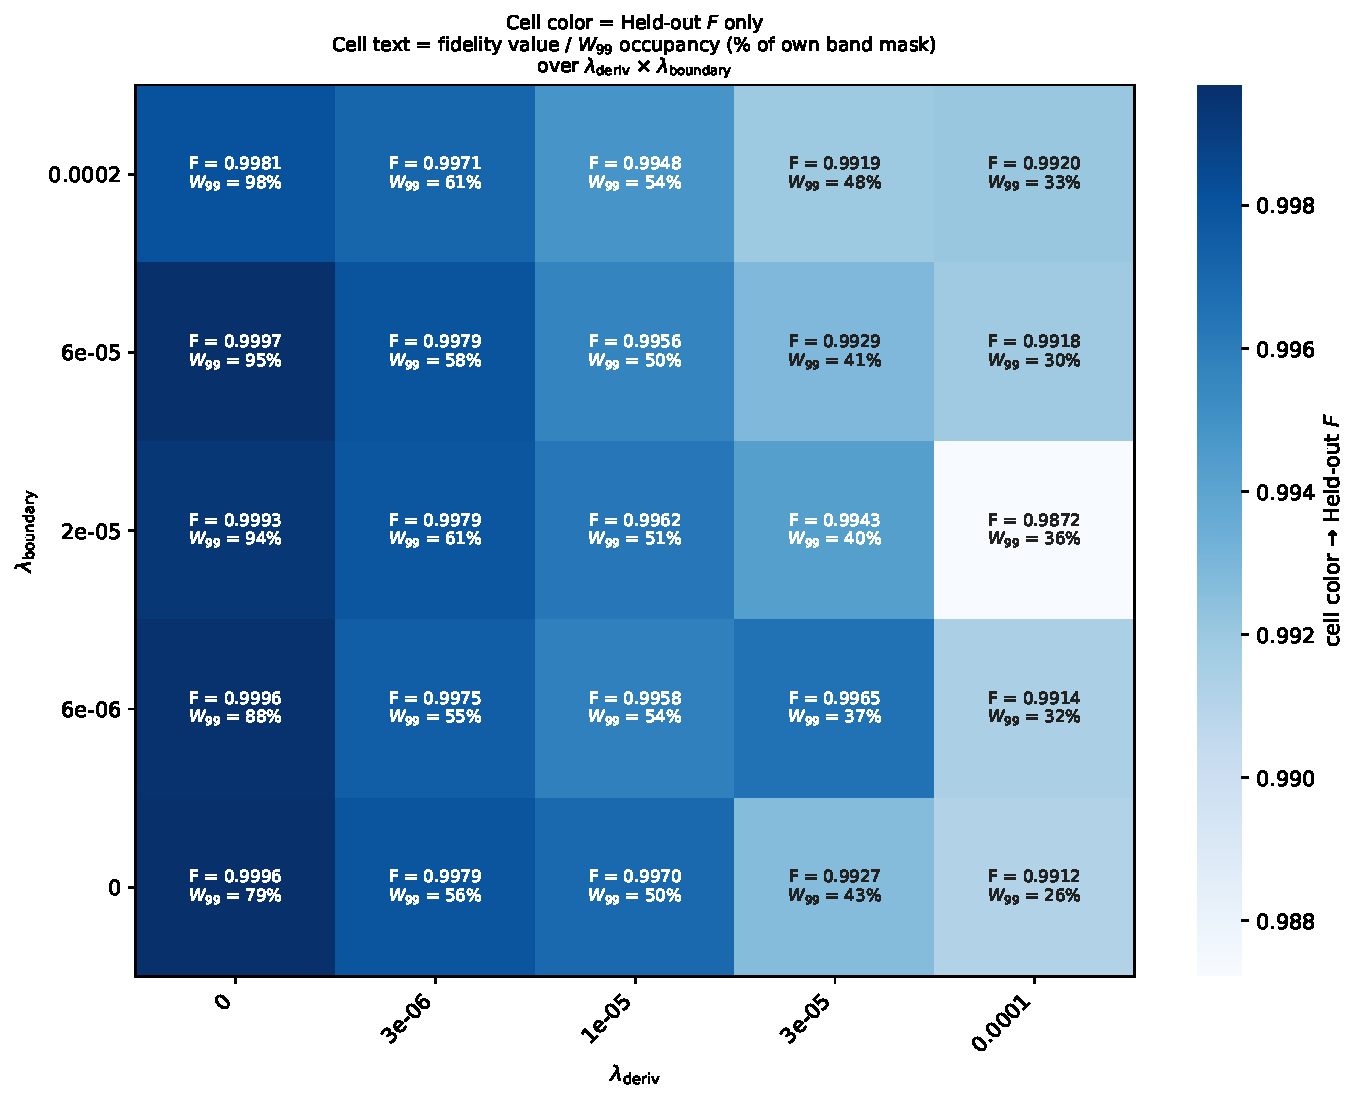
\includegraphics[width=0.85\textwidth]{figures/penalty_grid_heatmap.pdf}
    \caption{Held-out Pedersen fidelity over the two-dimensional
    $\lamd \times \lamb$ grid, with the RMS bandwidth annotated in each cell. The color ramp
    is single-hue sequential: it encodes magnitude, not polarity.}
    \label{fig:grid}
  \end{figure}
}{\emph{[Figure \texttt{figures/penalty\_grid\_heatmap.pdf} not found --- run the grid sweep.]}}

The grid uses the two axes that measurably move the pulse. $\lamd$ controls waveform smoothness
and therefore bandwidth; $\lamb$ controls how hard the drive is pinned to zero at the pulse
edges, which constrains the same waveform through a different mechanism, so an interaction
between them is plausible. A $\lamd \times \lamdisc$ grid was the original design, but by
Section~\ref{sec:inert} it would be constant along the $\lamdisc$ axis.

\subsection{Pareto front and the budgeted recommendation}

\IfFileExists{figures/penalty_pareto.pdf}{%
  \begin{figure}[htbp]
    \centering
    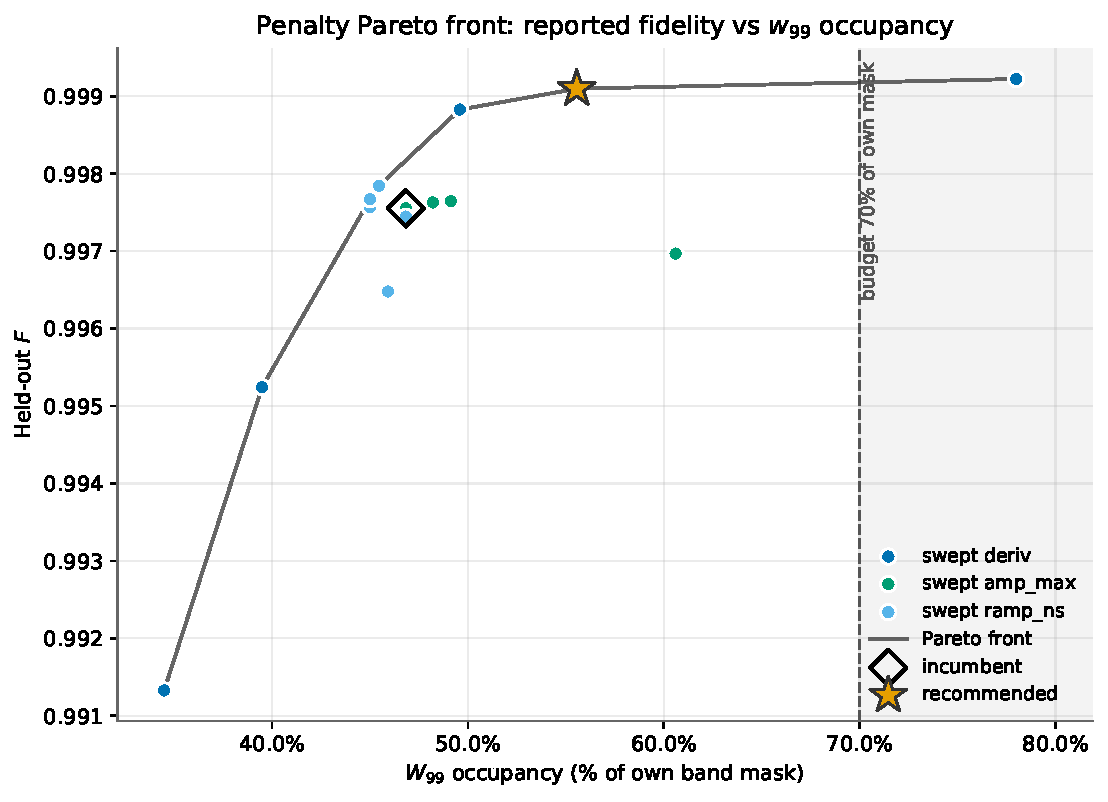
\includegraphics[width=0.85\textwidth]{figures/penalty_pareto.pdf}
    \caption{Reported held-out fidelity against RMS pulse bandwidth. A configuration is on the
    front when no other is simultaneously narrower in bandwidth and higher in fidelity. The
    shaded region lies outside the bandwidth budget; the star marks the recommendation, and the
    open diamond the incumbent recipe.}
    \label{fig:pareto}
  \end{figure}
}{\emph{[Figure \texttt{figures/penalty\_pareto.pdf} not found --- run the sweep.]}}

The selection rule is deliberately simple and stated in advance, so it cannot be retrofitted to
whatever the data happened to show: \emph{among configurations whose mean RMS bandwidth is within
the budget, take the highest mean held-out Pedersen fidelity; break ties toward lower
bandwidth.} The budget is a property of the control hardware, not of the optimization, which is
why it enters as a constraint rather than as another term in Eq.~\eqref{eq:cost}.

\subsection{Summary table}

\IfFileExists{tables/penalty_sweep_summary.tex}{%
  \begin{table}[htbp]
    \centering
    \small
    % Auto-generated by visualization/penalty_viz.summary_table -- do not hand-edit.
% cost statistic: occ99_frac   budget: 70% of own mask
\providecommand{\penaltybudget}{}%
\renewcommand{\penaltybudget}{$W_{99} \leq 70\%$ of each drive's own band mask}%
\setlength{\tabcolsep}{3.5pt}%
\begin{tabular}{llllllllllllll}
\toprule
$\lambda_{\mathrm{d}}$ & $\lambda_{\mathrm{b}}$ & $\lambda_{\mathrm{disc}}$ & $\epsilon_{\max}$ & $F_{\mathrm{held}}$ & $F_{\min}$ & $W_{99}^{C}$ & $W_{99}^{T}$ & binding & $\sigma_f$ & $\langle f\rangle_T$ & $\bar n_{\mathrm{drv}}$ & peak & in budget \\
\midrule
1e-06 & 2e-05 & 0.5 & 40 & 0.99924 & 0.99738 & 47\% & 59\% & tra & 9.04 & -8.91 & 4.06 & 21.7 & \checkmark \\
3e-06 & 2e-05 & 0.5 & 40 & 0.99868 & 0.99506 & 44\% & 53\% & tra & 8.24 & -6.79 & 3.10 & 20.2 & \checkmark \\
3e-06 & 0 & 0.5 & 40 & 0.99849 & 0.99238 & 41\% & 52\% & tra & 7.85 & -6.73 & 3.07 & 20.1 & \checkmark \\
3e-06 & 6e-06 & 0.5 & 40 & 0.99845 & 0.99233 & 45\% & 51\% & tra & 7.90 & -6.30 & 2.87 & 21.9 & \checkmark \\
3e-06 & 6e-05 & 0.5 & 40 & 0.99795 & 0.99100 & 47\% & 58\% & tra & 9.92 & -7.03 & 3.21 & 22.0 & \checkmark \\
1e-05 & 2e-05 & 0.5 & 40 & 0.99794 & 0.99411 & 38\% & 46\% & tra & 6.84 & -4.78 & 2.18 & 20.1 & \checkmark \\
1e-05 & 0 & 0.5 & 40 & 0.99778 & 0.99342 & 35\% & 46\% & tra & 6.90 & -5.37 & 2.45 & 19.1 & \checkmark \\
1e-05 & 2e-05 & 0.5 & 28 & 0.99775 & 0.99423 & 42\% & 48\% & tra & 6.91 & -5.29 & 2.41 & 19.9 & \checkmark \\
1e-05 & 2e-05 & 0.5 & 20 & 0.99771 & 0.99406 & 42\% & 48\% & tra & 6.93 & -5.30 & 2.42 & 19.7 & \checkmark \\
1e-05 & 2e-05 & 0.5 & 16 & 0.99761 & 0.99423 & 43\% & 49\% & tra & 7.21 & -5.12 & 2.33 & 17.9 & \checkmark \\
1e-05 & 2e-05 & 0.5 & 12 & 0.99751 & 0.99486 & 40\% & 52\% & tra & 7.64 & -6.24 & 2.85 & 15.0 & \checkmark \\
1e-05 & 2e-06 & 0.5 & 40 & 0.99747 & 0.99433 & 38\% & 47\% & tra & 6.84 & -5.44 & 2.48 & 18.7 & \checkmark \\
\bottomrule
\end{tabular}

    \caption{Penalty configurations ranked by held-out Pedersen fidelity, budget-feasible rows
    first. $\lambda_{\mathrm{d}}, \lambda_{\mathrm{b}}, \lambda_{\mathrm{a}}$ abbreviate the
    derivative, boundary, and amplitude weights. Generated by
    \texttt{visualization.penalty\_viz.summary\_table}.}
    \label{tab:summary}
  \end{table}
}{\emph{[Table \texttt{tables/penalty\_sweep\_summary.tex} not found --- run Section 6 of the
notebook.]}}

\section{Caveats}
\label{sec:caveats}

\paragraph{The held-out set includes under-resolved truncations.}
The scoring range extends down to $n_c = 16$, which does not fully contain the
$\alpha = \sqrt{3}$ cat ($\bar{n} = 3$). Those low truncations depress the held-out mean and
dominate the robustness spread for \emph{every} recipe, including good ones. They are kept
because a pulse that exploits the truncation wall fails there first --- that is exactly the
failure this sweep exists to detect --- but the absolute value of $F_{\mathrm{held}}$ should not
be quoted as ``the gate fidelity.'' The per-truncation breakdown in the manifest JSON is the
honest view.

\paragraph{Bandwidth here is a cost proxy, not a hardware specification.}
\texttt{bandwidth\_MHz} is an RMS spectral width, useful for ranking candidates against each
other. It is not an occupied-bandwidth or $-\SI{3}{\decibel}$ figure. The genuinely hard
frequency constraint is the band-limit projection inside the optimizer
(\texttt{core/fourier\_cutoff.py}), which is enforced by construction and is never violated
regardless of the penalty weights.

\paragraph{Seed variance is part of the result.}
The optimizer is non-convex and warm-started randomly. Differences in held-out fidelity smaller
than the across-seed standard deviation reported in Table~\ref{tab:summary} do not establish that
one recipe beats another.

\paragraph{The recommendation is per-gate.}
The sweep is run for one logical gate at a time. A recipe selected on $X$ is a reasonable
starting point for the other gates, not a validated setting for them.

\section{Reproducing}
\label{sec:repro}

\begin{lstlisting}
# OFAT ladder over all four penalties
python analysis/penalty_sweep.py --gate X --mode ofat \
       --seeds 42 7 123 --maxiter 1500

# Focused 2-D grid
python analysis/penalty_sweep.py --gate X --mode grid \
       --grid-x deriv --grid-y boundary --seeds 42 7 123 --maxiter 1500

# Figures, budgeted recommendation, and tables
#   -> set BW_BUDGET in penalty_optimization.ipynb, run with RUN_SWEEP = False
\end{lstlisting}

Both trained pulses and scored metric rows are disk-cached under
\texttt{results/penalty\_sweep\_cache/}, keyed by a hash of the full configuration, so an
interrupted sweep resumes without retraining and re-scoring never re-optimizes.

\end{document}
